\documentclass[11pt]{article}

\usepackage{graphicx}
\usepackage{latexsym}
\usepackage{setspace}
\usepackage{multicol}
\usepackage{caption}
\usepackage[utf8]{inputenc}
% \usepackage[T1]{fontenc}
\usepackage{tabularx, booktabs}
\usepackage{float}
\usepackage[textwidth=4cm]{todonotes}
\usepackage[normalem]{ulem}
\usepackage{graphicx}
\usepackage[toc,page]{appendix}

\restylefloat{figure}
\restylefloat{table[H]}

\newcolumntype{Y}{>{\centering\arraybackslash}X}

\begin{document}

\title{Multimodal annotation scheme for online written conversation analysis}

\begin{titlepage}

\maketitle

\tableofcontents

\end{titlepage}

\section{Introduction}

\subsection{Objects and definitions}

The objects of our study are computer-mediated - or "online" - written conversations. This includes conversations taking place through a number of mediums, such as web forums, message boards, mailing lists, chatrooms, and website comment sections. It excludes all forms of oral speech, as well as their transcripts. It also excludes all forms of offline written speech, such as the dialogues between characters in a book, journalistic interviews or messages written in a guestbook. 

\subsubsection{Participants, messages and subjects}

The conversations as we define them have three main characteristics:

\begin{itemize}
	\item Multiple \textit{participants}: a conversation is interactive by definition, and we define participants as human beings as well as bots taking actively part in the conversation by contributing new content and alterning between the roles of speaker and addressee.
	\item Multiple \textit{messages}: a conversation is built of several messages from various participants, and we define messages as the smallest technical unit of communication handled by the given medium (e.g. in a forum, posts are messages, in a mailing list, emails are messages, etc.).
	\item A \textit{subject}: conversations revolves around defined subjects, which are \textit{not} necessarily the formally defined subject lines or forum thread names (easily extracted from metadata), but rather the underlying motivation behind the conversation: i.e., what it is \textit{about}.
\end{itemize}

\subsubsection{Dialogues, polylogues and roles}

There is an important distinction between \textit{dialogues}, conversations between two participants, and \textit{polylogues}, conversations between two participants \textit{or more}.

Usually, in corpora constituted exclusively of dialogues, each participant has a well defined \textit{role}. For example, one may be a customer service agent and the other one a customer. In these scenarios, roles are static and remain the same through many conversations. Moreover, these conversations are often private: no one can "jump in" and send messages. But in other, more general corpora, where anyone can participate in a conversation, roles are not as well defined and can fluctuate during a conversation. It is however true in most cases that the conversation initiator (i.e. the first participant to send a message) is likely to be the one with the problem and thus the only one who can define it, acknowledge solutions for it and actually act on it in the real world.

As of now, the annotation scheme does not explicitely disinguish one from the other. From this point on in this document, we use the word "dialogue" to refer to both kinds of conversations.

\subsubsection{Problems and solutions}

We are more specifically interested in a more particular kind of conversation: functional conversations, i.e. conversations that are designed to convey information in order to help achieve an goal. When the motivation behind a conversation is to find solutions to a stated problem, we consider them to be problem/solution oriented conversations. They have a clearly stated goal and can be \textit{resolved}. These are at the heart of our research goals.
\newline
\newline
We define problems and solutions as follows:

\begin{itemize}
	\item Problem: an unwelcome matter or situation affecting one or several participants, that is considered harmful or needs to be resolved or worked around.
	\item Solution: a way of solving or working around a specific problem previously introduced in the conversation, usually in the first message of the thread.
\end{itemize}

\subsection{Goals}

Our goal is to develop an annotation scheme and protocol for the classification of message fragments in problem/solution oriented online conversations. The scheme should facilitate the problem/solution oriented analysis of message text, which, in turn, can be used for a number of applications:

\begin{itemize}
	\item Problem/solution oriented information retrieval (e.g. finding relevant documentation for a problem stated in natural language)
	\item Solution finding (e.g. the proposal of previous solutions that worked for a similar problem)
	\item Cross-modal analysis (e.g. using data from different sources to improve the efficiency of other tasks)
	\item Modality/channel relevance estimation (e.g. assisting users in finding the best place to find help)
	\item Etc.
\end{itemize}

Such a scheme would need to be:

\begin{itemize}
	\item Multimodal: applicable to different online mediums
	\item Exhaustive: capable of covering the entire text of a message
	\item Unambiguous: annotation should be made simple by following a decision tree
	\item Problem/solution oriented: useful in modelizing problems and their proposed solutions
\end{itemize}

A further objective is to use such annotated data to produce a sample segmentation of our email corpus so that we can test the validity of the hypotheses made in \cite{hernandez2014exploiting}.

% \section{Background}

% In this section we introduce the concept of dialog act (DA).

% \subsection{Speech Acts}

Speech act theory \cite{austin1975things} attempts to describe utterances in terms of communicative function (e.g. question, answer, thanks...). Indeed, utterances are not limited to their semantic content, they also have a communicative function : a goal, and an effect. For Austin, they can be analyzed at three levels: locutory (the linguistic characteristics of the utterance), illocutory (the intention of the speaker) and perlocutory (the real-world effects of the utterance). When we refer to speech acts\footnote{Also known as dialog acts in the context of interactive conversations}, we are interested in the illocutory level of utterance analysis. 

Thus, in most works, it is in terms of speech acts that interactions between participants of a conversation are modeled. Austin considers utterances as actions performed by a speaker ; this is based on the idea that every enunciation is the realization of a social act. Verbs that specify these actions are called \textit{performative verbs}, such as when someone says "I grant you the title of captain". But speech acts are not only constituted by these kinds of verbs. \cite{searle1976taxonomy} offers five classes of dialog acts : assertives (assertion...), directives (order, request, advice, etc.), commissives (promise, invitation, etc.), expressives (congratulations, thanks, etc.) and declarations (war declaration, nomination, baptism, etc.).

There are a number of different speech act taxonomies \cite{traum200020}. Two of them can be considered foundational: first Austin's and then Searle's. Both contain five classes of speech acts, that can be defined as such:

% \todo{Réécrire définitions (en l'état copié/collé Wikipédia)}

\begin{itemize}
	\item Assertives: speech acts that commit a speaker to the truth of the expressed proposition, e.g. reciting a creed.
	\item Directives: speech acts that are to cause the hearer to take a particular action, e.g. requests, commands and advice.
	\item Commissives: speech acts that commit a speaker to some future action, e.g. promises and oaths.
	\item Expressives: speech acts that express the speaker's attitudes and emotions towards the proposition, e.g. congratulations, excuses and thanks.
	\item Declaratives: speech acts that change the reality in accord with the proposition of the declaration, e.g. baptisms, pronouncing someone guilty or pronouncing someone husband and wife.
\end{itemize}

Table \ref{fig:fundamentalTaxonomies} provides examples of these two taxonomies. Table \ref{fig:emailTaxonomies} presents a few more recent taxonomies specifically used in the context of online conversation analysis.

\begin{table}
	\begin{tabularx}{\textwidth}{c c c}
		\toprule
		\cite{austin1975things} & \cite{searle1976taxonomy} & Examples \\
		\midrule
		Verdictives & Declarations & To condemn, decree... \\
		Exercitives & Directives & To command, order, forgive... \\
		Commissives & Commissives & To promise, guarantee, bet, swear... \\
		Behabitives & Expressives & To apologize, thank, criticize... \\
		Expositives & Assertives & To assert, deny, postulate... \\
		\bottomrule
	\end{tabularx}
	\caption{Foundational taxonomies for speech acts categorization}
	\label{fig:fundamentalTaxonomies}
\end{table}

\begin{table}
	\begin{tabularx}{\textwidth}{c c c}
		\toprule
		ActS & Corpus & Reference \\
		\midrule
		Disclosure &  & \\
		Edification &  & \\
		Advisement &  & \\
		Confirmation & Multi-domain & \cite{Lampert_classifyingspeech} \\
		Question &  & \\
		Acknowledgment &  & \\
		Interpretation &  & \\
		Reflection &  & \\
		\midrule
		Direct request &  & \\
		Question-request &  & \\
		Open question &  & \\
		First person commitment & Corporate email & \cite{de2013classification} \\
		First person expression of feeling &  & \\
		First person other &  & \\
		Other statements &  & \\
		\midrule
		Accept response &  & \\
		Acknowledge and appreciate &  & \\
		Action motivator &  & \\
		Polite mechanism &  & \\
		Rhetorical question &  & \\
		Open-ended question & BC3 & \cite{JanAAAI08} \\
		Or/or-clause question &  & \\
		Wh-question &  & \\
		Yes-no question &  & \\
		Reject response &  & \\
		Statement &  & \\
		Uncertain response &  & \\
		\bottomrule
	\end{tabularx}
	% \todo[inline]{À enrichir}
	\caption{Examples of speech act taxonomies specific to online conversation analysis}
	\label{fig:emailTaxonomies}
\end{table}

% \subsection{Verbal Response Modes}

\todo[inline]{Ajouter quelques paragraphes sur les VRM}

% \section{Bibliography}

% \todo[inline]{Ajouter un paragraphe introductif + tableau qui restitue les différents travaux entre eux (par domaine, corpus, schéma, tâche, approche...)}

% \subsection{Online written conversation analysis}

% \subsubsection{Sentence classification in message board posts}

Here we explain the work of \cite{qadir2011classifying}. Their research is relevant to our work because of their goal - to classify sentences as speech acts in online messages, because of their data - web forum posts, and because of their taxonomy - which is based on speech acts.

\vspace{0.5cm}
\textbf{Goals:}
\vspace{0.1cm}

The authors work with message board posts. They consider that not all sentences carry a speech act. Their primary goal is to distinguish between those that do and those that don't (which they call \todo{Mieux définir "expository", positionner le terme par rapport aux expositives d'Austin et les assertives de Searle}\textit{expository sentences}). Their second goal is to classify speech act sentences into four types: \textit{commissives}, \textit{directives}, \textit{expressives} and \textit{representatives}. These four classes are derived from the work of \cite{searle1976taxonomy}. Searle's fifth type of speech acts, \textit{declarations}, was omitted because the authors found almost no examples of it in their corpus. \todo{Expliquer dans le texte pas dans une table} This taxonomy is further explained in Table \ref{fig:qadirTaxonomies}.

Their ultimate objective is to develop a system capable of classifying sentences in a topic-independent manner (the data they worked with was extracted from forums dealing with veterinary medicine).

\begin{table}
	\begin{tabularx}{\textwidth}{c l}
		\toprule
		Class & Definition \\
		\midrule
		Expository Sentence & Presents or explain information to the reader \\
		\midrule
		Commissive & Contains a stated commitment from the author \\
		Directive & Contains an expectation that readers will do something as a response \\
		Expressive & Contains a statement of the author's psychological state \\
		Representative & Commits the author to the truth of a certain proposition \\
		\bottomrule
	\end{tabularx}
	\caption{Taxonomy used in \cite{qadir2011classifying}}
	\label{fig:qadirTaxonomies}
\end{table}

\vspace{0.5cm}
\textbf{Message board specificities:}
\vspace{0.1cm}

According to the authors, speech acts occur differently in message board posts than in spoken dialog. 

They found that while the most common everyday occurrences of \textit{commissives} are promises and threats, it is not so in forum data. Most occurrences of this type of speech act correspond to confirmations that the participant will perform some action in the future. The authors also consider that declarations from the participant that they will not do something are sentences carrying such a speech act.

They found that \textit{directive} speech acts are common in message board posts, in particular under the form of a question or a request for assistance or advice. They attempt to weed out rhetorical questions from sentences classified as \textit{directives}.

The authors found that typical examples of \textit{expressive} speech acts occur when a participant thanks, welcomes or apologizes to a reader. They found this class to be very common in message board posts.

\textit{Representative} speech acts were uncommon in the corpus they used. They chose to ignore most sentences stated as fact even though they might correspond to Searle's definition of a representative speech act and and label them as \textit{expository sentences} instead. They considered that sentences belonged in that class only when a doctor explicitly presented an opinion or hypothesis as their own (such as sentences starting with "I suspect that...").

\vspace{0.5cm}
\textbf{Classification:}
\vspace{0.1cm}

The authors chose to approach the problem as a supervised classification task. Instead of a single classifier, they chose to train four different binary models, one for each class, and run them against the data. Therefore a single sentence can contain several speech acts. A preliminary classifier was trained just to filter out sentences containing no speech act (\textit{expository sentences}).

They use a number of different feature sets for the classification task. First, they consider lexical and syntactic features. Such features include: unigrams, personal pronouns, tense, modals, plan phrases, punctuation, sentence position, number of verbs, and others. Second, they consider speech act word clues. In \cite{searle1976taxonomy}, the author listed a number words that he considered to be indicative of speech acts. Here, the authors chose to discard a few that they considered too general and added new ones, such as a list of speech act verbs originally published by \cite{wierzbicka1987english}. Their system recognize all derivations of these word clues.

The classifiers used were Support Vector Machines (SVMs).

\vspace{0.5cm}
\textbf{Evaluation:}
\vspace{0.1cm}

The data set used was constituted of 15,383 message board posts from the Veterinary Information Network (VIN)\footnote{www.vin.com}. These posts covered three topics: cardiology, endocrinology, and feline internal medicine. The preprocessing included number tokenization, the removing of html tags and "basic cleaning" (???). Experiments were performed on a random sample of 150 threads from the collection. These threads contained 1,956 sentences (13.04 sentences per post).

The gold standard was built from the manual annotation of message posts by two human annotators provided with detailed annotation guidelines. A sample of 50 posts was independently annotated by them in order to calculate the annotator agreement. However, the authors ran into the same problem \cite{kim2010taggingandlinking} did, that is the fact that the standard Cohen's Kappa is not applicable to multi-class annotation tasks. Since they found only a small number of sentences classified as containing several speech acts, these were discarded and the kappa was calculated for the rest. The result was a score of .95, an extremely high agreement. However the "no speech act" class was by far the most predominant (70\%), so the kappa score does not necessarily mean that annotators mostly agreed on speech act classification decisions. The authors therefore computed the kappa for each speech act class and found an average score of 87.25\%, which is still very high. Table \ref{fig:qadirRepartition} shows the repartition of speech acts in their dataset.

\begin{table}
	\begin{tabularx}{\textwidth}{Y Y}
		\toprule
		Class & Proportion \\
		\midrule
		None & 71.42\% \\
		Directive & 15.90\% \\
		Expressive & 9.92\% \\
		Representative & 2.91\% \\
		Commissive & 2.61\% \\
		\bottomrule
	\end{tabularx}
	\caption{Repartition of speech acts in \cite{qadir2011classifying} test data}
	\label{fig:qadirRepartition}
\end{table}

The first classifier, the one filtering out sentences containing no speech act, recognized 83\% of the speech act sentences with 86\% precision, and 95\% of the expository  sentences with 93\% precision. As for the speech act categorization task, the authors performed many experiments with a number of different feature combinations, for each speech act category. The authors found that many syntactic and lexical features had little impact on the classification results. Detailed results will not be presented here, but overall results were good for the identification of directive and expressive speech act sentences, less so for representative and commissive speech acts, which proved more difficult to detect.

% \subsubsection{Speech act classification applied to forum posts}

Here we explain the work of \cite{kim2010taggingandlinking}. Their research is relevant to our work because of their goal (to link and classify messages) and their corpus (email messages). Their taxonomy, however, is not based on dialog acts.

\vspace{0.5cm}
\textbf{Methodology:}
\vspace{0.1cm}

The authors annotate both threads and posts in a corpus built from the CNET forums\footnote{http://forums.cnet.com}. Two annotators use a dedicated tool\footnote{http://mandrake.csse.unimelb.edu.au/~rbp/cgi-bin/su/Classify.py} for the annotation task. Before starting to annotate the overall data set, a pilot annotation was performed to ensure that both annotators had the same understanding of the taxonomy.

\vspace{0.5cm}
\textbf{Taxonomy:}
\vspace{0.1cm}

First, they classify threads into two groups of classes: the basic group, which is further subdivided into \textit{Solution Type} classes and \textit{Problem Source} classes, as well as a miscellaneous group. The different classes are detailed in table \ref{fig:threadClasses}. \textit{Solution Type} and \textit{Problem Source} classes can be used either separately or together, therefore there is an additional combined class set made of each combination of a \textit{Solution Type} class and a \textit{Problem Source} class (e.g. \textit{Search-OS} or \textit{Install-Network}). The combined class set being the superset of basic class sets, it was used to do the annotation.

\begin{table}
	\begin{tabularx}{\textwidth}{Y Y}
		Class & Group \\
		\toprule
		Support & Solution Type \\
		Documentation & Solution Type \\
		Install & Solution Type \\
		Search & Solution Type \\
		\midrule
		Hardware & Problem Source \\
		Operating System & Problem Source \\
		Software & Problem Source \\
		Media & Problem Source \\
		Network & Problem Source \\
		Programming & Problem Source \\
		\midrule
		Spam & Miscellaneous \\
		Other & Miscellaneous \\
		\bottomrule
	\end{tabularx}
	\caption{Thread classes in \cite{kim2010taggingandlinking}}
	\label{fig:threadClasses}
\end{table}

Then, they annotate each individual post with one or several post classes. These classes are categorized into two groups, the answer group and the question group, plus three single classes. The different classes used are detailed in table \ref{fig:postClasses}.

\begin{table}
	\begin{tabularx}{\textwidth}{Y Y}
		Class & Group \\
		\toprule
		Answer-Answer & Answer \\
		Answer-Add & Answer \\
		Answer-Correction & Answer \\
		Answer-Confirmation & Answer \\
		Answer-Objection & Answer \\
		\midrule
		Question-Question & Question \\
		Question-Add & Question \\
		Question-Correction & Question \\
		Question-Confirmation & Question \\
		\midrule
		Resolution & - \\
		Reproduction & - \\
		Other & - \\
		\bottomrule
	\end{tabularx}
	\caption{Post classes in \cite{kim2010taggingandlinking}}
	\label{fig:postClasses}
\end{table}

\vspace{0.5cm}
\textbf{Annotator agreement:}
\vspace{0.1cm}

The authors use Cohen's Kappa to compute annotator agreement:

$$\kappa = \frac{P(a) - P(e)}{1 - P(e)}$$

Where $P(a)$ refers to the relative observed agreement between two annotators, and $P(e)$ is the hypothetical probability of chance agreement between two annotators.

However, as they write: "\textit{The standard Cohen’s Kappa cannot be used in multi-class annotation tasks. By the time the annotation process started, no standard methodology for calculating Cohen’s Kappa for multi-class tasks was found. Therefore, an extended method for calculating $\kappa$ value was proposed to address this problem.}"

They propose an improved Cohen's Kappa for a multi-class situation, but the methodology is not applicable to our case because it takes into account the link information for each class (a concept we do not consider at all).

\vspace{0.5cm}
\textbf{Classification:}
\vspace{0.1cm}

The authors use four different models for thread classification: 1 Nearest Neighbor, Naïve Bayes and Support Vector Machine. A majority class model (ZeroR) and a random model (RAND) are used as baselines. Features are weighed using four different schemes: Information Gain (IG), Term Frequency-Inverse Document Frequency (TF-IDF), raw count and simple binary. For post classification, the authors use a conventional Maximum Entropy learner\footnote{http://maxent.sourceforge.net/} as well as two structural learners : SVM-HMMs and CRFs (using \emph{CRF++}\footnote{http://crfpp.sourceforge.net/
})

Features for threads are built by using the initial post or concatenating all posts in the thread to form the "text" of the thread. They then construct different bag-of-words feature sets by tuning different parameters such as input text, pre-processing, tokenization method, and $n$-gram length. For posts, features used include lexical, structural, contextual, and semantic features.

\vspace{0.5cm}
\textbf{Evaluation:}
\vspace{0.1cm}

Results for both thread classification and post classification are evaluated using micro-average precision ($P_{\mu}$), recall ($R_{\mu}$), F-score ($F_{\mu}$) and macro-averaged precision ($P_{M}$), recall ($R_{M}$) and F1-score ($F_{M}$) on a stratified\footnote{The authors make sure that \textit{"if a given post is contained in the test data for a given iteration, all other posts in that same thread are also in the test data (or more pertinently, not in the training data)"}} 10-fold cross-validation.

% \subsubsection{Segmentation of email message text}

Here we explain the work of \cite{lampert2009segmenting}. It is relevant to our work because of their goal, which is to classify sentences or text fragments as belonging to such or such message zone, and because of the kind of data they work with: email messages.

\vspace{0.5cm}
\textbf{Goals:}
\vspace{0.1cm}

The authors attempt to segment emails into several prototypical areas, called \textit{email zones}. They call their system "Zebra".

\vspace{0.5cm}
\textbf{Email zones:}
\vspace{0.1cm}

There are three superclasses containing nine different classes of email zones.

\textit{Sender zones} contain text written by the current sender. This superclass contains the following subclasses: \textit{author} (new content by the sender), \textit{greeting} (polite greetings at the beginning of a message), and \textit{signoff} (closing words of a message).

\textit{Quoted conversation zones} include content quoted from other messages. The subclasses for this superclass are: \textit{reply} (content quoted from a previous message in the thread) and \textit{forward} (content from an email outside the thread that has been forwarded by the current sender).

\textit{Boilerplate zones} contain reusable message content, typically automatically appended to a message. Subclasses include: \textit{signature} (contact information automatically appended at the end of a message), \textit{advertising} (advertising material, typically found at the end of the message), \textit{disclaimer} (legal disclaimers and privacy statements), and \textit{attachment} (automated text indicating attached documents).

\vspace{0.5cm}
\textbf{Classification:}
\vspace{0.1cm}

The authors consider that each line of text in the body of a message belongs to one of these \textit{email zones}. The authors tried two approaches: in the first one, a classifier segments a message into zone fragments and then attempts to classify the resulting fragments. In the second approach, the classifier simply works on a line-by-line basis.

In the first approach, the fragment-based one, the message is segmented based on detected \textit{zone boundaries}. These boundaries are identified thanks to what the authors call "buffer lines", i.e. blank lines or lines containing only whitespace or punctuation characters.

The classifier is based on SVMs (Support Vector Machines) and uses graphic, orthographic and lexical features to categorize lines and text fragments.

\vspace{0.5cm}
\textbf{Evaluation:}
\vspace{0.1cm}

The training data for their classifier consists of almost 400 messages from the Enron email corpus \cite{klimt2004enron}. To build the gold standard, the authors chose to use only a single annotator since they believe the task to be relatively uncontroversial. Each line - blank lines excepted - was marked by the annotator as belonging to one of the nine zones. They used the resulting 7,922 annotated lines (out of 11,881) as training data for their classifier.

The results are calculated by 10-fold cross-validation. 

The zone boundary detection system (used for the fragment based approach) reaches 90\% accuracy.

Concerning zone classification, interestingly, the line-based approach outperformed the fragment-based one by a small margin, probably due to the 10\% of inaccuracies in boundary detection. Zebra obtains a 91.53\% accuracy for the classification of lines into the three superclasses, and 87.01\% in all nine classes.

% \subsection{Dialog act taxonomies}

% \subsubsection{The DAMSL taxonomy for dialog annotation}



% \subsubsection{DIT++ for functional markup}



\newpage

\section{Proposal}

% Here we describe our findings and proposal.

% \subsection{General classes}

These classes are mutually exclusive and must cover the entire text. Therefore each sentence belong to one and only one of these classes. Child nodes are specialisations of their parents, the sum of the scopes of all child nodes is not equal to the scope of the parent.

\vspace{0.5cm}
\textbf{Content}
\vspace{0.1cm}

Sentences are considered to be ``content'' if they were written or manually included expressely for the considered message.

\begin{itemize}
	\item Dialog acts (see subsection \ref{subsec:dialog_acts} for details)
	\item Structure
		\begin{itemize}
			\item Markup
			\item Framing text
				\begin{itemize}
					\item Heading
					\item ...
				\end{itemize}
		\end{itemize}
\end{itemize}

\textbf{Boilerplate}
\vspace{0.1cm}

Sentences are considered as ``boilerplate'' if they have been or are intended to be reused by the author. ``Boilerplate'' sentences frame the message.

\begin{itemize}
	\item History
	\item Signature
	\item Advertisement
	\item Disclaimer
	\item Contact information
\end{itemize}

This taxonomy of dialogue acts is derived from DIT++\cite{bunt2009dit++}.

\subsection{Concept definitions}
\label{subsec:dialogue_acts}

\subsubsection{Dialogue acts}

\begin{figure}
	\caption{Meta-model}
	\centering
	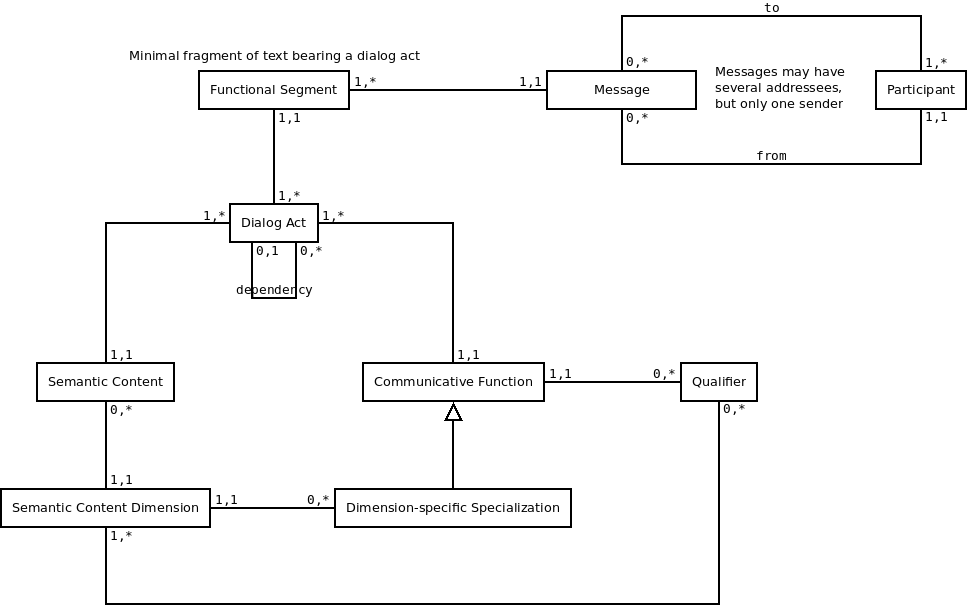
\includegraphics[keepaspectratio,width=0.6\paperwidth]{figures/objects.png}
	\label{fig:metaModel}
\end{figure}

In the "information-state update" (also know as "context-change") approach to dialogue analysis, dialogue acts are interpreted as update operations applied to the information states of the interacting participants \cite{traum2003information,bunt2011semantics}. In this perspective, they are defined here as the conjunction of two components: a \textit{semantic content} and a \textit{communicative function} (see figure \ref{fig:fundamentalTaxonomies}).

The former, the semantic content, specifies the objects, propositions, and all the things that the dialogue act is about, and therefore contains all the information used in the update operation. The latter, the communicative function, specifies the way the dialogue act is intended to impact the information state of the addressee. For example, the utterance "do you know what time it is?" is about the time that it is - that's its semantic content - but its communicative function could be either a genuine question (the speaker doesn't know the time but wants to find out) or a reproach (the speaker noticed the addressee is late and is upset about it).

A functional segment is defined as the minimal fragment of text bearing a dialogue act and is hereafter used interchangeably with the term "utterance".

\subsubsection{Dimensions in dialogue act annotation}

Human communication is a complex activity. In functional conversations, there is often a certain activity or task which the participants want to perform through the dialogue and as a result is the focus most interactions. In conversations bearing requests for assistance, this task is to solve problems. However, people do not communicate only to reach the formal objectives of the conversation, they also constantly monitor the communicative process, synchronize their mutual understanding through feedback utterances, respect social conventions such as greeting and thanking, etc. Often, utterances can be multifunctional and may serve several purposes related to several of these things. For example, in the following exchange:

\begin{enumerate}
	\item P1: Comment est ce que j'installe Dia ?
	\item P2: Tout simplement : apt-get install dia
	\item P1: Ça me dit permission non accordée je fais quoi ? 
	\item P3: Essaye avec sudo devant la commande
	\item P1: C'est bon merci !
\end{enumerate}

In the third utterance, participant 1 does two things: firstly, he informs his audience that he ran into an issue, and, secondly, he asks for further instructions. In the fifth utterance, he does two things again: he signifies that his problem is solved, and he also thanks the participants that helped him.

Such multi-functionality implies that accurate annotation of utterances with dialogue act information calls for the assignment of more than one tag to an utterance. This process is called "multi-label annotation". However in most multi-label schemes, only a small percentage of possible tag combinations are actually used, due to the fact that many tags are in fact mutually exclusive. This is an issue because it makes both human annotation and machine classification harder by unnecessarily increasing the task's complexity.

Here, like in DIT++, we guide annotators and classification algorithms in not considering impossible label combinations by the use of a multidimensional annotation scheme \cite{bunt2006dimensions}. The scheme allows each utterance to be annotated with one of 14 mutually exclusive tags per \textit{semantic dimension}. Semantic dimensions are defined as the different areas within which dialogue acts can be semantically categorized.

For example, if the communicative function of the fragment "C'est bon merci !" for a dimension called "social management" is "express gratitude", it cannot be any other in the same dimension, but it can be another in a different one, like "indicate problem solved" in the dimension "task management" for example.

\subsection{Taxonomy}

\subsubsection{Dimensions}

For this scheme, we define six semantic dimensions:

\begin{itemize}
	\item Communication: dialogue acts about the communication process (e.g. \textit{"J'ai fait une faute de frappe dans mon précédent mail c'est grep pas gret"})
	\item Discourse: dialogue acts affect both the discourse's structure and the topics discussed (e.g. \textit{"Avant de vous expliquer mon problème, j'ai un coup de gueule à faire passer"})
	\item Social Obligations: dialogue acts that take care of social conventions such as thanks, greetings, apologies etc. (e.g. \textit{"Merci beaucoup !!!!"})
	\item Auto Feedback: dialogue acts related to the speaker's own processing of an utterance (e.g. \textit{"Perso j'ai rien compris"})
	\item Allo Feedback: dialogue acts related to the addressee(s)'(s) processing of an utterance (e.g. \textit{"Je sais pas si je suis très clair...?"})
	\item Task: dialogue acts that bring information about the task's objects, i.e. problems, solutions, goals, user profiles, contexts, etc. (e.g. \textit{"Mon problème c'est que j'ai même pas l'icône dans le systray"})
\end{itemize}

\subsubsection{Communicative functions}

Here we define the fourteen general communicative functions of the scheme. As was said before, they are all mutually exclusive. At most one per dimension can be attributed to the same functional segment. A segment can therefore bear up to six dialogue acts, however, in most cases, there is only one act per utterance, sometimes two, and rarely three or more.

These functions are sufficient to cover any utterance on any dimension.

Labels are written in capital letters, other items in the following bullet lists are merely function categories and subcategories, not to be used for annotation. 

\vspace{0.25cm}

\textbf{Information Transfer}
\vspace{0.1cm}

Information transfer functions deal with the exchange of information between participants.

\begin{itemize}
	\item Direct Information Transfer:
		\newline These functions are neither backward nor forward looking, they provide information that was not directly elicited by a previous utterance.
		\begin{itemize}
			\item $ASSERT$: if the speaker is the source of the information
			\newline \textit{"Une nouvelle version d'Opera est sortie la semaine dernière."}
			\item $QUOTE$: if the speaker is not the source of the information
			\newline \textit{"version : commande introuvable"}
		\end{itemize}
	\item Information Transfer Elicitation:
		\newline These functions are forward-looking, they create an expectation for new information.
		\begin{itemize}
			\item $ASK$: if the speaker expects another participant to provide the information
			\newline \textit{"Comment ça se fait ?"}
			\item $SELF-ASK$: if the speaker is creating the expectation only to answer it himself (like a rhetorical question, for example)
			\newline \textit{"Problème réglé ? Eh ben non !"}
		\end{itemize}
	\item Information Transfer Feedback:
		\newline These functions are backward-looking, they provide information that relates to a previously uttered dialogue act.
		\begin{itemize}
			\item $ANSWER$: if the information was directly elicited by a previous utterance that had a forward-looking information transfer function
			\newline \textit{"C'est probablement parce que tu as oublié d'installer latex-mk"}
			\item $REACT$: if the information was not directly elicited
			\newline \textit{"Ça me paraît pas très propre ta solution"}
		\end{itemize}
\end{itemize}

\textbf{Action planning}
\vspace{0.1cm}

Action planning functions deal with the management of the participants' actions. 

\begin{itemize}
	\item Direct Action Planning
		\newline These functions are neither backward nor forward looking, they either commit the speaker to an action or direct the addressee.
		\begin{itemize}
			\item $COMMIT$: commits the speaker to an action
			\newline \textit{"Je m'en charge"}
			\item $DIRECT$: directs the addressee to perform an action
			\newline \textit{"Signale le bug sur le tracker Mantis"}
		\end{itemize}
	\item Action Planning Elicitation:
		\newline These functions are forward-looking and elicit the addressees' approval of an action plan.
		\begin{itemize}
			\item $OFFER$: if the action is to be performed by the speaker
			\newline \textit{"Je peux revérifier si tu veux"}
			\item $REQUEST$: if the action is to be performed by the addressee
			\newline \textit{"Est ce que tu peux poster le contenu de ton fichier .bashrc?"}
		\end{itemize}
	\item Action Planning Feedback:
		\newline These functions are backward-looking and address an action planning elicitation function
		\begin{itemize}
			\item $ADDRESS$ $REQUEST$: if the action is to be performed by the speaker
			\newline \textit{"Non c'est mort je n'ai même pas envie d'essayer"}
			\item $ADDRESS$ $OFFER$: if the action is to be performed by the addressee
			\newline \textit{"Ah oui stp je veux bien que tu t'en charges"}
		\end{itemize}
\end{itemize}

\textbf{Other}
\vspace{0.1cm}

\begin{itemize}
	\item Performative Locution
		\newline This function is not only describing a given reality but also actively changing it.
		\begin{itemize}
			\item $DECLARE$: the utterance of a dialogue act having this function is, at least in part, an attempt at doing an action
			\newline \textit{"J'abandonne"}
		\end{itemize}
	\item Self Expression
		\newline This function expresses the speaker's psychological state, or his psychological position towards something.
		\begin{itemize}
			\item $EXPRESS$: 
			\newline \textit{"Merci beaucoup !"}
		\end{itemize}
\end{itemize}

\subsection{Extensions}

While the six semantic dimensions and the fourteen communicative functions defined above are sufficient to cover virtually any conversation, more information may be necessary to effectively achieve more specific tasks, such as the modelization of problems and solutions in conversations bearing requests for assistance, or following the evolution of the mood a participant during his interactions.

\subsubsection{Dialogue act dependencies}

Our taxonomy of communicative functions includes several forward-looking and backward-looking functions that fall in either the information transfer or the action planning categories of functions. The former create an expectation (of information, of agreement, etc.) while the latter may satisfy these expectations. Being able to represent these expectations and to know whether they were satisfied or not would require the annotation of relational information about communicative functions. This is done by marking relationships between backward-looking functions and the utterance they relate to. By doing this, we can easily detect unsatisfied demands: there is one for each utterance bearing a forward-looking function that is not linked to a backward-looking dialogue act (or that is linked only to a partial backward-looking act).

The annotation of dialogue act dependencies in the Task dimension would be very useful in evaluating a problem-solving process.

\subsubsection{Function qualifiers}

Up to this point our annotation allow us to know what an utterance is \textit{about} (the semantic content's dimension) and how it should be \textit{processed} (the act's communicative function). However, additional data on utterances would be useful to reach an additional level of understanding of the dialogue. 

\cite{petukhova2010introducing} introduces the notion of \textit{qualifier}, that are used in conjunction with communicative functions to describe the utterance more precisely. They propose a representation of dialogue behaviour expressing intentions with different possible qualifications, relating to uncertainty, conditionality, partiality and mode.

The four qualifiers are:

\begin{itemize}
	\item Modality: epistemic modal qualifiers specify the strength of the speaker's belief about the truth of a proposition (only information transfer functions are concerned by this qualifier)
	\item Conditionality: they represent the ability, necessity or volition of performing actions (only action planning functions are concerned by this qualifier)
	\item Partiality: they limits the scope of the communicative function to only a part of the dialogue act to which the current segment is related (only backward-looking functions are concerned by this qualifier)
	\item Mode: broad category of qualifiers concerned with the speaker's attitude and emotional state
\end{itemize}

For simplicity, we treat modality, conditionality and partiality qualifiers as binary values. Respectively, these values are: "certain" or "uncertain", "conditional" or "unconditional", and "partial" or "complete". There are several taxonomies available in the literature that could be used to label emotional and attitudinal phenomena in dialogue, however we choose to stay at a coarse level of granularity and use only "positive", "negative" and "neutral" as possible values for the mode qualifier.

To illustrate the use of qualifiers, let's take the following exchange as an example:

\begin{enumerate}
	\item P1: Est ce que Unity et Gnome 3 sont disponibles sous Debian ?
	\item P2: Il me semble que Unity n'est dispo que sous Ubuntu
	\item P1: Bon si j'ai le temps ce week end je passerai sous Gnome alors
\end{enumerate}

Using the previous qualifiers, it could be annotated as such:

\begin{enumerate}
	\item Task: Ask
	\item Task: Answer[partial, uncertain]
	\item Task: Commit[conditional]
\end{enumerate}

\subsubsection{Problem and solution sub-objects}

Problems and solutions are complex objects with a variety of properties. To be able to model them with increased accuracy, we may define the following sub-objects:

\begin{itemize}
	\item Problem
		\begin{itemize}
			\item $SYMPTOMS-DESCRIPTION$: description of the problem and how it affects the user and the system\\
			\textit{"Le software-center crash au lancement"}
			\item $GOAL-STATEMENT$: what the participant wants, but is prevented to achieve by the problem\\
			\textit{"J'aimerais bien utiliser Unity sous Debian"}
			\item $CONTEXT$: relevant information about the state of the world when the problem occurred\\
			\textit{"Je suis sous Ubuntu 12.04"}
			\item $CONTEXT-UPDATE$: relevant update concerning the state of the world\\
			\textit{"Maintenant j'arrive même plus à lancer le dashboard"}
		\end{itemize}
	\item Solution
		\begin{itemize}
			\item $SOLUTION-INSTRUCTION$: the steps that are to be followed to solve the problem\\
			\textit{"Redémarre ton PC"}
			\item $SOLUTION-ENTITY$: the "thing" that needs to be acquired to solve the problem and that embodies the solution, may imply a solution-instruction\\
			\textit{"J'ai besoin d'écrire en dictant mon texte", "Utilise Dragon Natural Speaking"}\\
			\item $SOLUTION-EXPLANATION$: the explanation of a problematic behaviour that implies a solution-instruction, may imply a solution-instruction\\
			\textit{"C'est parce que tu n'as pas lancé la commande en root"}\\
			\item $SOLUTION-CONSTRAINT$: specifications on the solution by the participant(s) experiencing the problem\\
			\textit{"J'ai pas envie d'avoir à tout réinstaller"}
			\item $SOLUTION-LIMITATION$: description of the solution's limits and shortcomings, as well as doubts about it's validity\\
			\textit{"Par contre c'est payant..."}
		\end{itemize}
\end{itemize}

The annotation of utterances of the Task dimension with these items, done in the same manner as if they were qualifiers, would be extremely useful. For example:

\begin{enumerate}
	\item P1: Etant cloué au lit depuis un accident j'aurais aimé savoir si on peut utiliser la reconnaissance vocale sous linux ?
	\item P1: Je suis sous Ubuntu 12.04
	\item P1: Merci pour votre aide
	\item P2: Il doit exister une licence professionnelle de Dragon Naturally Speaking
	\item P3: Oui mais elle est sans doute très chère, et pas libre...
\end{enumerate}

Could be annotated in the following manner:

\begin{enumerate}
	\item Task: Assert\{Goal-Statement\}
	\item Task: Assert\{Context\}
	\item Social Obligations: Express
	\item Task: Assert[uncertain]\{Solution-Entity\}
	\item Task: React\{Solution-Limitation\}
\end{enumerate}

With that information, two objects can be created and their different attributes "filled" with semantic information:

\begin{itemize}
	\item Problem 1:
		\begin{itemize}
			\item Goal: to use vocal recognition on linux
			\item Context: a system operating Ubuntu 12.04
		\end{itemize}
	\item Solution 1:
		\begin{itemize}
			\item Solution-Entity: the software "Dragon Naturally Speaking"
			\item Limitations: it's expensive, it's proprietary
		\end{itemize}
\end{itemize}

\subsubsection{Dimension-specific function specializations}

In order to allow a more subtle definition of dialogue acts, their communicative function can be specialized into a dimension-specific label. These labels are all an extension of one of the fourteen general functions.

Assigning a function specialization is entirely optional, they are not necessary to annotate the text ; however they help in understanding how the semantic content of an utterance can be used. For example, it is useful to differentiate between a greeting and a farewell, even if both of the acts are declarations of the social obligations' dimension.

The following list is not exhaustive and subject to change.

\begin{itemize}
	\item Assert
		\begin{itemize}
			\item Social Obligations
				\begin{itemize}
					\item $SELF-INTRODUCE$
						\newline \textit{"Moi c'est Danny je viens de m'inscrire sur la liste"}
				\end{itemize}
			\item Auto Feedback
				\begin{itemize}
					\item $PROVIDE$ $FEEDBACK$
						\newline \textit{"J'ai rien compris !"}
				\end{itemize}
			\item Allo Feedback
				\begin{itemize}
					\item $PROVIDE$ $FEEDBACK$
						\newline \textit{"J'ai pas l'impression que tu aies bien compris"}
				\end{itemize}
			\item Task
				\begin{itemize}
					\item $REPORT$
						\newline \textit{"J'ai essayé d'utiliser le software-center mais ça a crashé au milieu de l'installation"}
					\item $DESCRIBE$
						\newline \textit{"Je suis sous Ubuntu 12.10"}
					\item $CONSTRAINT$
						\newline \textit{"Je préfererais ne pas avoir à réinstaller Ubuntu"}
					\item $ENOUNCE$ $LIMITATION(S)$
						\newline \textit{"Par contre c'est payant"}
				\end{itemize}
		\end{itemize}
	\item Quote
		\begin{itemize}
			\item Task
				\begin{itemize}
					\item $LINK$ $RESOURCE$
						\newline \textit{"https://help.ubuntu.com/lts/ubuntu-help/unity-launcher-intro.html"}
					\item $SHARE$ $OUTPUT$
						\newline \textit{"E: Impossible d'ouvrir le fichier verrou /var/lib/dpkg/lock"}
				\end{itemize}
		\end{itemize}
	\item React
		\begin{itemize}
			\item Task
				\begin{itemize}
					\item $APPRAISE$
						\newline \textit{"Ça ne marchera jamais"}
				\end{itemize}
		\end{itemize}
	\item Ask
		\begin{itemize}
			\item Auto Feedback
				\begin{itemize}
					\item $ELICIT$ $FEEDBACK$
						\newline \textit{"Du coup il faut que je recommence tout, c'est bien ça ?"}
				\end{itemize}
			\item Allo Feedback
				\begin{itemize}
					\item $ELICIT$ $FEEDBACK$
						\newline \textit{"T'as compris ce que je voulais dire ?"}
				\end{itemize}
			\item Task
				\begin{itemize}
					\item $ELICIT$ $APPRAISAL$
						\newline \textit{"Je pense que ça devrait marcher, est ce que quelqu'un peut confirmer ?"}
				\end{itemize}
		\end{itemize}
	\item Request
		\begin{itemize}
			\item Task
				\begin{itemize}
					\item $REQUEST$ $HELP$
						\newline \textit{"Donc si vous pouviez me donner des conseils ce serait sympa"}
				\end{itemize}
		\end{itemize}
	\item Address Request
		\begin{itemize}
			\item Task
				\begin{itemize}
					\item $ANNOUNCE$ $TRIAL$
						\newline \textit{"J'essaye dès que je rentre à la maison"}
				\end{itemize}
		\end{itemize}
	\item Declare
		\begin{itemize}
			\item Communication
				\begin{itemize}
					\item $SWITCH$ $CHANNEL$
						\newline \textit{"Tant pis je vais demander sur le forum ce sera plus simple"}
				\end{itemize}
			\item Discourse
				\begin{itemize}
					\item $PRECLOSE$
						\newline \textit{"Bon perso je vais pas tarder à y aller"}
					\item $OPEN$
						\newline \textit{"bip Popaul j'ai une question si t'es toujours là"}
					\item $INTRODUCE$ $TOPIC$
						\newline \textit{"J'aimerais bien qu'on se refocalise sur Gnome 3 perso"}
					\item $SHIFT$ $TOPIC$
						\newline \textit{"Pour en revenir à Unity..."}
				\end{itemize}
			\item Social Obligations
				\begin{itemize}
					\item $GREET$
						\newline \textit{"Bonjour tout le monde"}
					\item $FAREWELL$
						\newline \textit{"A+"}
				\end{itemize}
			\item Task
				\begin{itemize}
					\item $FORFEIT$
						\newline \textit{"J'abandonne"}
					\item $UPDATE$ $STATUS$
						\newline \textit{"Ok c'est bon ça marche !"}
				\end{itemize}
		\end{itemize}
	\item Express
		\begin{itemize}
			\item Social Obligations
				\begin{itemize}
					\item $EMOTE$
						\newline \textit{";-)"}
					\item $WISH$
						\newline \textit{"Bonne soirée !"}
					\item $DOWNPLAY$
						\newline \textit{"Mais de rien"}
					\item $THANK$
						\newline \textit{"Merci beaucoup !"}
					\item $APOLOGIZE$
						\newline \textit{"Vraiment désolé..."}
				\end{itemize}
		\end{itemize}
\end{itemize}

% \subsection{Speech Act Classes}
\label{subsec:speech_act_classes}

The \textbf{speech act} superclass contains four subclasses: \textbf{assertives}, \textbf{commissives}, \textbf{directives} and \textbf{expressives}. 

They are derived from the five classes defined in \cite{searle1976taxonomy} (the fifth class, "declarations", was omitted because we assume it will almost never appear in our corpus: \cite{qadir2011classifying} found almost no example of it in their datasets).

\vspace{0.3cm}
\textbf{Assertives}
\vspace{0.1cm}

Assertives are sentences that commit a speaker to the truth of the expressed proposition.

\begin{itemize}
	\item Subjective report: account of something the author has observed, heard, done, or investigated
		\begin{itemize}
			\item Action report: reporting of actions taken (e.g. \textit{"I did try apt-cache search geotiff but it didn't work", "I upgraded my system to 10.04 via clean install"})
			\item Result report: reporting of the results of actions taken (e.g. \textit{"I did try apt-cache search geotiff but it didn't work", "No such luck"})
				\begin{itemize}
					\item Solution research result report: specific type of result report pertaining to the search for a solution (e.g. \textit{"I couldn't find anything on the forums"})
				\end{itemize}
			\item Observation: a remark, statement, or comment based on something one noticed ("It doesn't happen every time I move the cursor, it is completely random")
		\end{itemize}
	\item Objective report: exact reporting of something without author interpretation
		\begin{itemize}
			\item Computer text: copy-and-paste of code, log, or commands (e.g. \textit{"usermod - G admin 2ndroot"})
			\item Quote: exact copy of a portion of text with an indication that one is not the original author
		\end{itemize}
	\item Statement: definite and clear expression of the nature or truth of something
	\item Description: objective account of a system, person or event
		\begin{itemize}
			\item Event description: description of an event
			\item System description: retranscription of a system's settings or specifications (e.g. \textit{"My ubuntu 1 bandwidth settings are set to -1", "I am using ubuntu 12.04"})
			\item Author profile: description of the author's identity, habits, experiences, preferences or skills (e.g. \textit{"Coming from a Windows world, I've probably been spoiled but..."})
		\end{itemize}
	\item Assimilation: expression of a belief in the similarity or non-similarity of two things
		\begin{itemize}
			\item Assertion: a confident and forceful statement of fact (e.g. \textit{"DD will work over the network", "Even OS X has nothing close to it, unfortunately"})
			\item Guess: estimate or supposition without sufficient information to be sure of being correct (e.g. \textit{""}).
			\item Correction: rectification of an alleged error or inaccuracy
		\end{itemize}
\end{itemize}

\textbf{Commissives}
\vspace{0.1cm}

Commissives are sentences containing a stated commitment from the author.

\begin{itemize}
	\item Acknowledgment-Commitment: a commitment to do something in reaction to a previous message in the thread (e.g. \textit{"Ok thanks I'll try that as soon as I get home", "Hopefully it's explained in detail in there, I will search..."})
	\item Channel change: announcement that the author is going to switch or fork the conversation to a different communication channel (e.g. \textit{"I'll file a wishlist bug for this"})
\end{itemize}

\textbf{Directives}
\vspace{0.1cm}

Directives are sentences containing an expectation that readers will do something as a response.

\begin{itemize}
	\item Question: a sentence worded or expressed so as to explicitly elicit information (e.g. \textit{"Should I just change them by hand?", "Is there anyway to recover these short of recreating everything from scratch and restoring from backup?"})
		\item Clarification request: request for more specific information or confirmation that the author has correctly understood an utterance (e.g. \textit{"do you mean the starterbar from gdesklets?", "Which exact packages are you getting an error from?"})
	\item Request for assistance: call for help (e.g. \textit{"please help!", "can anyone help me???", "i could use some help"})
	\item Suggestion: an idea submitted for consideration
	\item Instruction: information telling how something should be done (e.g. \textit{"Open a terminal"})
\end{itemize}

\textbf{Expressives}
\vspace{0.1cm}

Expressives are sentences containing a statement of the author's psychological state.

\begin{itemize}
	\item Greeting: polite words of salutation
		\begin{itemize}
			\item General greeting: greeting directed to no one in particular (e.g. \textit{"Hi all", "Hello all"})
			\item Targeted greeting: greeting directed at a specific participant or group of participants (e.g. \textit{"Hey Steve"})
		\end{itemize}
	\item Signoff: the conclusion of a message (e.g. \textit{"see you", "-best - greg"})
	\item Thanks: an expression of gratitude
		\begin{itemize}
			\item Thanks in advance: an expression of anticipated gratitude (e.g. \textit{"Thanks for any help,"})
			\item Thanks in reaction: an expression of gratitude for some specific assistance (e.g. \textit{"Thanks I'll try that!"})
		\end{itemize}
	\item Opinion: expression of a subjective judgment on a thing or situation (e.g. \textit{"what a nightmare", "this is bullshit", "this OS sucks"})
		\begin{itemize}
			\item Feedback: specific type of constructive opinion destined to be used as a basis for the improvement of a product or service
		\end{itemize}
	\item False question: question whose function is not to elicit an answer
		\begin{itemize}
			\item Rhetorical question: question asked in order to make a point (e.g. \textit{"Are you seriously implying that he should reinstall Ubuntu because of a cosmetic issue?", "Wow, CRTs to store data?"})
			\item Personal interrogation: question asked in order to express a sentiment (e.g. \textit{"I wonder how it works?", "Come on, how hard can this be?"})
		\end{itemize}
	\item Expression of solution confidence: expression of the author's level of confidence in a proposed solution (e.g. \textit{"I don't know much about it, I just discovered it on gnomefiles.org", "However, it may do what you need"})
	\item Expression of solution preference: expression of the author's preferences (to varying degree) towards a specific type of solution
\end{itemize}

% \subsection{Problem/Solution Classes}

The following taxonomy aims at capturing the way conversation participants introduce, explain and communicate about these problems and solutions.

The whole text doesn't have to be classified into these classes. Some sentences don't belong in any of them. 

\subsubsection{Primary Classes}

In online conversations bearing expressions of need and attempts at answering to those needs, we consider that sentences may bear information on two types of abstract objects

These two classes are mutually exclusive.

\begin{itemize}
	\item Problem
	\item Solution
\end{itemize}

\subsubsection{Secondary Classes}

These classes define the kind of information a sentence brings about a problem or a solution.

These classes are not mutually exclusive

\begin{itemize}
	\item Definition
		\begin{itemize}
			\item Statement
					\begin{itemize}
						\item Problem statement
						\item Goal statement
						\item Question
						\item Expression of solution preference
					\end{itemize}
			\item Correction
			\item Explanation
		\end{itemize}
	\item Reception
		\begin{itemize}
			\item Confirmation
			\item Assimilation
				\begin{itemize}	
					\item Problem assimilation
				\end{itemize}
			\item Acknowledgement
				\begin{itemize}
					\item Acknowledgment-Commitment
					\item Trial report
				\end{itemize}
			\item Refutal
			\item Appraisal
				\begin{itemize}
					\item Rhetorical question
					\item Expression of solution confidence
				\end{itemize}
			\item Resolution
		\end{itemize}
\end{itemize}

\newpage

\begin{appendices}

\chapter{Graphical representation of the taxonomy (attached file: $taxonomy.png$)}

\begin{figure}[H]
	\caption{Graphical taxonomy preview}
	\centering
	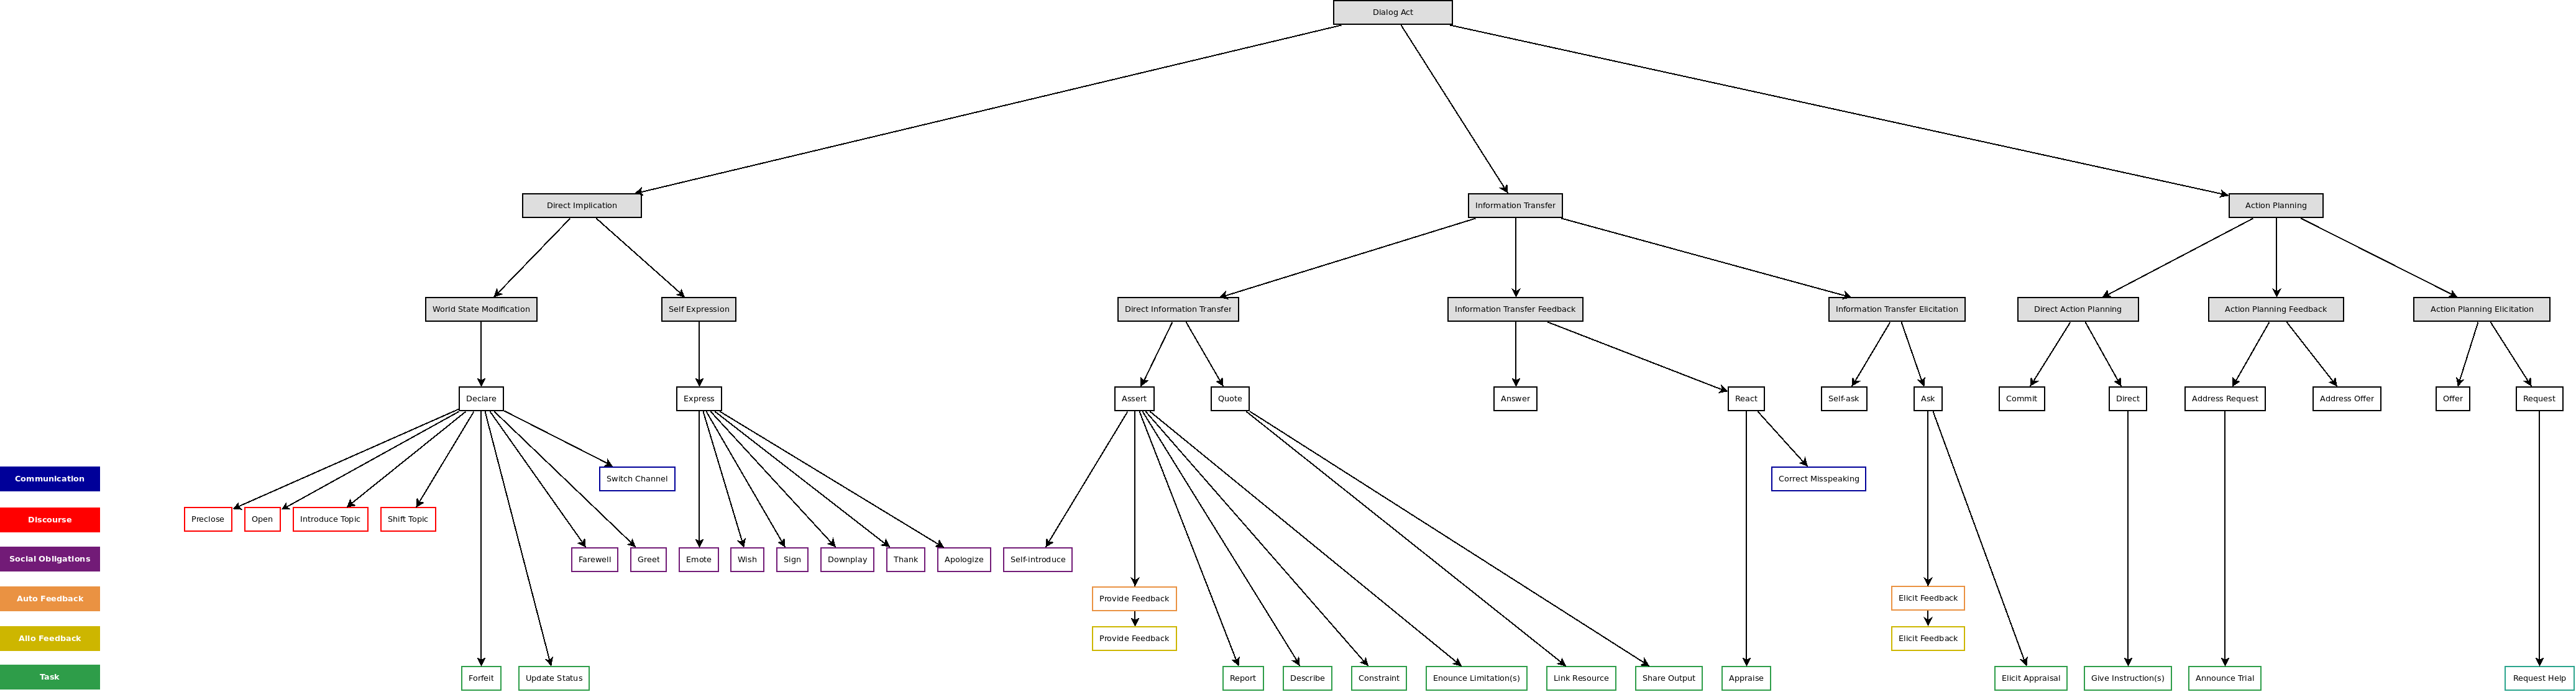
\includegraphics[keepaspectratio,width=0.6\paperwidth]{figures/taxonomy.png}
	\label{fig:taxonomy}
\end{figure}

\end{appendices}

\newpage

\bibliographystyle{apalike}
\bibliography{bibliography}

\end{document}
